

% Символы, специфичные для моей статьи по теории возможностей

\newcommand{\td}{т.\,д.}
\newcommand{\te}{т.\,е.}
\makeatletter

\usepackage{datatool, fp}

\def\showevColorOne{blue!50!black}
\def\showevColorHigh{blue!60}
\def\showevColorLow{blue!20}
\def\showevColorZero{white}

\def\showeval@basecolor{blue!70!black}

\newlength{\showeval@xshift}\setlength{\showeval@xshift}{5.5mm}
\newlength{\showeval@nodewidth}\setlength{\showeval@nodewidth}{5.5mm}
\newlength{\showeval@yshift}\setlength{\showeval@yshift}{4.5mm}
\newlength{\showeval@nodeheight}\setlength{\showeval@nodeheight}{3.5mm}

%%%%%%%%%%%%%%%%%%%%%%%%%%%%%%%%%%%%%%%%%%%%%%%%%%

\DTLnewdb{showeval@db}

\newcounter{showeval@counI}
\newcounter{showeval@counII}

%%%%%%%%%%%%%%%%%%%%%%%%%%%%%%%%%%%%%%%%%%%%%%%%%%

\def\showeval@drawticks{
    \foreach \showeval@point in {0, 1, 2, 3, 4, 5, 6, 7, 8, 9, 10} {
        \node[
            rectangle, \showevColorHigh,
            xshift=\showeval@point\showeval@xshift
        ]{\small\showeval@point};
    }
}

\def\showeval@drawticks@rough{
    \node[
        rectangle, \showevColorHigh,
        xshift=1\showeval@xshift,
        minimum width=3\showeval@xshift,
        text height=3mm, text depth=1mm
    ]{\small плохо};
    \node[
        rectangle, \showevColorHigh,
        xshift=5\showeval@xshift,
        minimum width=5\showeval@xshift,
        text height=3mm, text depth=1mm
    ]{\small средне};
    \node[
        rectangle, \showevColorHigh,
        xshift=9\showeval@xshift,
        minimum width=3\showeval@xshift,
        text height=3mm, text depth=1mm
    ]{\small хорошо};
}

\def\showeval@drawonebar@fullscale@fullrange#1{
    \foreach \showeval@point in {0, 1, 2, 3, 4, 5, 6, 7, 8, 9, 10} {
        \setcounter{showeval@counII}{\showeval@point+1}
        \def\showeval@pl{\csname showeval@p\Roman{showeval@counII}\endcsname}
        \FPeval{\showeval@density}{round(round(\showeval@pl * 10, 0) * 10, 0)}
        \node[
            rectangle, draw,
            minimum width=\showeval@nodewidth, minimum height=\showeval@nodeheight,
            white, fill=\showeval@basecolor!\showeval@density, draw=black,
            xshift=\showeval@point\showeval@xshift,
            yshift=#1
        ]{};
    }
}

\def\showeval@drawonebar@discrete@fullrange#1{
    \foreach \showeval@point in {0, 1, 2, 3, 4, 5, 6, 7, 8, 9, 10} {
        \setcounter{showeval@counII}{\showeval@point+1}
        \def\showeval@pl{\csname showeval@p\Roman{showeval@counII}\endcsname}
        \FPeval{\showeval@density}{round(\showeval@pl *3, 0)}
        \ifthenelse{\equal{\showeval@density}{0}}{\def\showeval@cur@color{\showevColorZero}}{}
        \ifthenelse{\equal{\showeval@density}{1}}{\def\showeval@cur@color{\showevColorLow}}{}
        \ifthenelse{\equal{\showeval@density}{2}}{\def\showeval@cur@color{\showevColorHigh}}{}
        \ifthenelse{\equal{\showeval@density}{3}}{\def\showeval@cur@color{\showevColorOne}}{}
        \node[
            rectangle, draw,
            minimum width=\showeval@nodewidth, minimum height=\showeval@nodeheight,
            white, fill=\showeval@cur@color,
            xshift=\showeval@point\showeval@xshift,
            yshift=#1
        ]{};
    }
}

\def\showeval@display#1#2#3{
    \DTLsetseparator{ }
    \DTLnewdbonloadfalse
    \DTLloaddb[
        noheader, 
        keys={p00,p01,p02,p03,p04,p05,p06,p07,p08,p09,p10}
    ]{showeval@db}{#1}
    \DTLnewdbonloadtrue
    \begin{tikzpicture}
        \ifthenelse{\equal{#3}{rough}}{\showeval@drawticks@rough}{\showeval@drawticks}
        \setcounter{showeval@counI}{0}
        \DTLforeach{showeval@db}{
            \showeval@pI   =p00,
            \showeval@pII  =p01,
            \showeval@pIII =p02,
            \showeval@pIV  =p03,
            \showeval@pV   =p04,
            \showeval@pVI  =p05,
            \showeval@pVII =p06,
            \showeval@pVIII=p07,
            \showeval@pIX  =p08,
            \showeval@pX   =p09,
            \showeval@pXI  =p10%
        }{
            \stepcounter{showeval@counI}
            \ifthenelse{\equal{#2}{full scale}}{%
                \showeval@drawonebar@fullscale@fullrange{-\value{showeval@counI}\showeval@yshift}%
            }{%
                \showeval@drawonebar@discrete@fullrange{-\value{showeval@counI}\showeval@yshift}%
            }
        }
    \end{tikzpicture}
    \DTLgcleardb{showeval@db}
}

\def\showevDisplayFullScale#1{\showeval@display{#1}{full scale}{full range}}
\def\showevDisplay#1{\showeval@display{#1}{discrete}{full range}}
\def\showevDisplayRough#1{\showeval@display{#1}{discrete}{rough}}

\makeatother


\title[Субъект. суждения и принятие решений]{Выбор наиболее качественных объектов на основе нечётких данных об их характеристиках}
\institute[Физфак МГУ]{Физический факультет МГУ имени~М.\,В.\;Ломоносова\\Кафедра информатики и чего-то там
       \\ \vspace{0.3cm}
      Научный руководитель:  Зубюк Андрей Владимирович \\ \vspace{0.5cm} }
\author{Борисов Кирилл}
%\url{kiraboris@gmail.com}

\date{19 ноября 2015~г.}
% \date{\today}

\begin{document}
\selectlanguage{russian}
\sloppy

% ==== first slide === 
\maketitle

\section{Проблематика выбора объектов}
\begin{frame}{C чем мы имеем дело?}
	%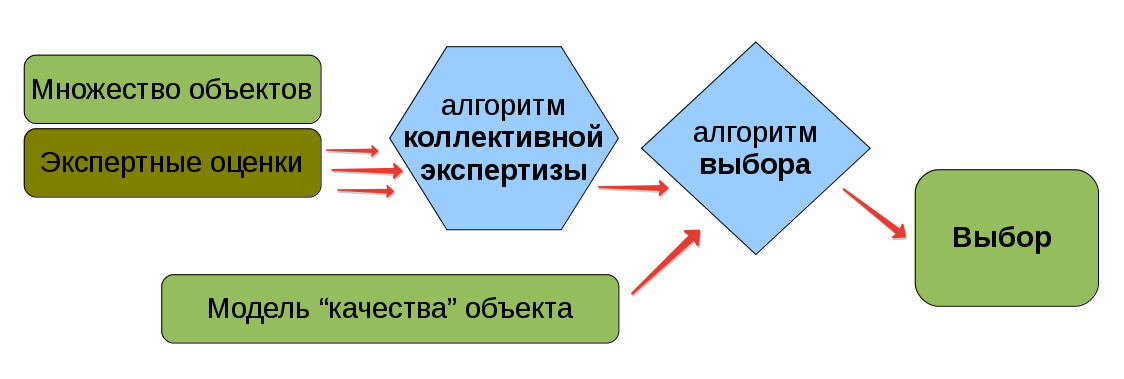
\includegraphics[width=0.8\linewidth]{./pic/globalscheme}
 	\begin{columns}
 		\column{0.50\textwidth}
 			Есть $n$ объектов, у каждого объекта % составителем методологии выбрано
 			есть $m$ параметров. Модель: {\small {\em независимые} нечёткие элементы} 
			\\ \vspace*{2mm}   % характеризуем с совсем разных сторон
 			$\tilde x_{ij} \in X$, {\footnotesize $i = 1 \ldots n$, $j = 1 \ldots m$} 
 			\\ \vspace*{3mm}
 			$x_{ij} \in X$ -- их значения (неизвестны), где $X$ --  числовое множество.
 			\\[1.1ex] {\small Например, $X = \{1, \ldots, 10\}$ --  множество баллов по десятибалльной шкале} 
 			%некое выпуклое подмножество действительной оси
 		\column{0.50\textwidth}
 			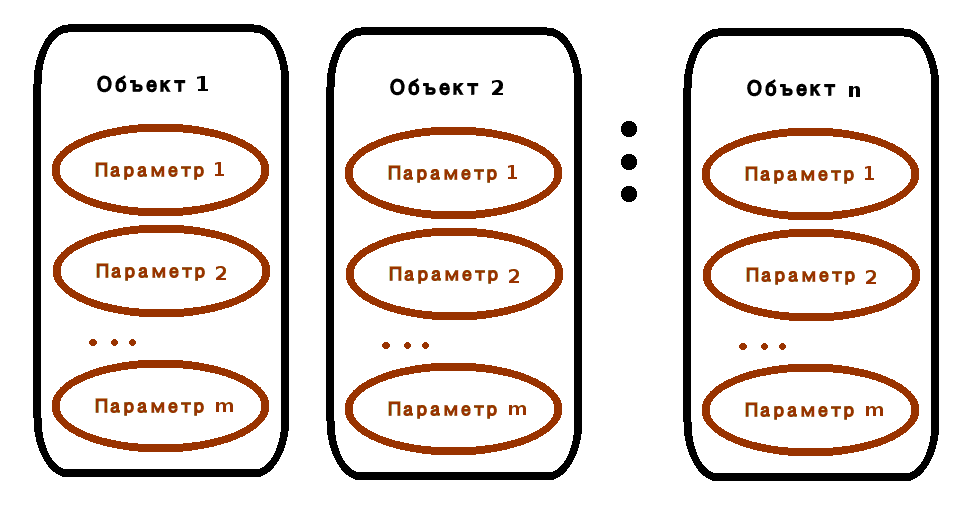
\includegraphics[width=1.0\linewidth]{./pic/theobjects}
 	\end{columns}
 	
	\vspace*{5mm}
	\begin{columns}
		\column{0.60\textwidth}
		Экспертные оценки -- это распределения $\tilde x_{ij}$: 
		{\large \begin{center} \hspace{-8mm}  $\p_{ij}^{(r)}( \cdot )$ \end{center} }
		{\footnotesize где $i = 1 \ldots n$ -- номер объекта, $j = 1 \ldots m$, -- номер параметра, $r = 1 \ldots R$ -- номер эксперта}.  
		\column{0.40\textwidth}
		\begin{center}
			\vspace*{-6mm}
			%   {\small Примеры оценок:}
			  {\scriptsize {Примеры оценок: значения $\p(x)$ показаны цветом, $x \in \setTen$}}
			  \\ \vspace*{2mm}
			  \resizebox{1.0\linewidth}{!}{\showevDisplayFullScale{./pic/chapter01-tech01.dat}}
		\end{center}
	\end{columns}

 \end{frame} %===========================

\begin{frame}{Процесс выбора объектов}
	 
	 \vspace*{-3ex}
	 \hspace{2mm} Модель <<качества>>  объекта:
	  \\[1ex] \hspace{25mm} { \small \tikz { \node  (n1) { \light{монотонна и задана заказчиком экспертизы}  }; } }
	 \\  \hspace{5mm}  $x_i = \tikz[baseline] { \node[anchor=base, fill=\mygreen] (t1) {$f$}; } (x_{i1}, ..., x_{im}),\; x_i \in X$ -- <<качество>> объекта с номером $i$; 
	 \\  \hspace{5mm} например, для $x_{i1}, x_{i2}$ можно взять $\displaystyle f(x_{i1}, x_{i2}) = \frac{1}{2} (x_{i1} + x_{i2})$. 
	\begin{tikzpicture}[overlay]
		\path[->] (n1.west) edge  (t1.north east);
	\end{tikzpicture}
	\vspace*{1ex}
	\begin{center}
	      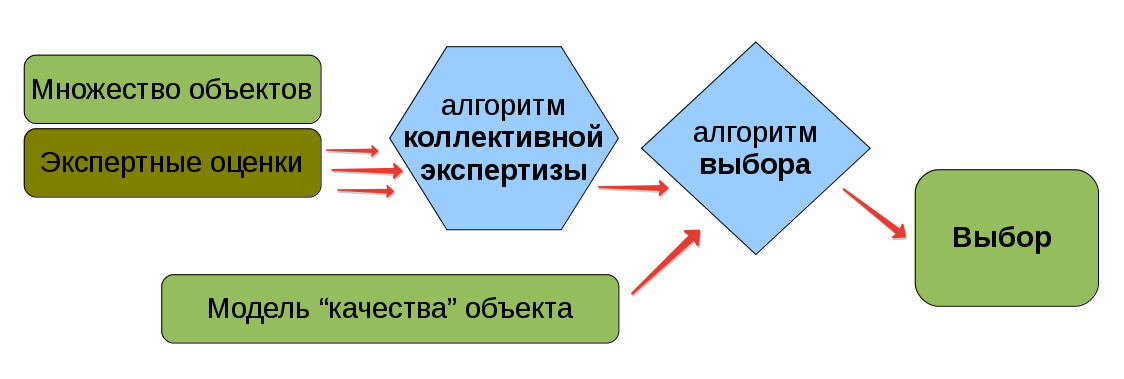
\includegraphics[width=0.9\linewidth]{./pic/globalscheme}
	\end{center}      
 \end{frame} %===========================
 
\section{Задача и алгоритм выбора}
\begin{frame}{Задача выбора объектов}
	
	{ Пусть $t = (x_{11}, ..., x_{nm}) \in T = X^{nm}$ -- вектор значений параметров всех объектов}.	
	 {\small Например, в случае $X = \{1, \ldots, 10\}$ размер пространства $\abs{T} = 10^{nm}$}. 
	\\[1.5ex] Пусть $d \subset \setN$ -- какой-то выбор; $\delta_t$ -- {\em верный} выбор {\small при известном $t$}. %нсли бы знали x_i
	\begin{gather*}
	      \abs{d} = \abs{\delta_t} = k \text{ -- задано; } \delta_{t} \define= \{i_1, \mydots, i_k\}: \forall\, i \in \delta_t,\; \forall\, i' \in \setN \setminus \delta_t: \\ f(x_{i1}, ..., x_{im}) > f(x_{i'1}, ..., x_{i'm}).
	 \end{gather*}
	%\vspace*{-2mm}
	\vspace{-4ex}
	\begin{center}
	 Работает \emph{один} эксперт {\small (или используется результат коллективной экспертизы)}.
	 
	Оценки $\p_{ij}$ %,{\footnotesize $i = 1 \ldots n$, $j = 1 \ldots m$},
	    порождают возможность $\P(\{t\}) = \p(t)$ через их совместное распределение $\p(x_{11}, \ldots, x_{nm}) = \inf_{i, j}\,\p_{ij}(x_{ij})$, {\footnotesize $i = 1 \ldots n$, $j = 1 \ldots m$}.
	    
	%\end{center}
	% каждый эксперт оценивает все параметры, которые являются разложением макропараметров качества объектов.
	% в данной задаче всюду используется одна и та же шкала возможности
	%\\ \vspace*{2mm} $\P(\{t\}) = \p(t)$.
	%\vspace*{-2mm}
	%\begin{center}
	%      \vspace*{-1mm}
	     \textbf{Задача }{\small (ставится впервые)}: \tikz[baseline] {  \node[anchor=base, fill=\mygreen]{ $\P(\Eps(d)) \sim \underset{d} \min$ }; },
	     где $\Eps(d) = \{d \neq \delta_t\}$. % размер подможества.
	     \\[1ex] {\footnotesize Оптимальное решение может быть не единственным!}
	\end{center}
\end{frame} %===========================

\begin{frame}{Алгоритм выбора: работа с  возможностью}
\vspace*{-4mm} 
\begin{gather*}
%	\text{\small Возьмем любое событие $A$, в частности, $A= \Eps(d)$.}
	%\hspace*{4mm} 
	\mathsmaller{  t = (x_{11}, \ldots, x_{nm})  \in T = X^{nm}, x_{ij} \text{ -- его коордианты}, {i = 1 \ldots n, j = 1 \ldots m}.}
	\\[2ex] \P(A) = \text{?..  перебрать все $t \in T$ можно за $O(\abs{X}^{nm})$ операций}.
	\\ \P(A) > p_0 \in \zo \text{?.. Решается за $O(nm)$ из-за свойств $\sup$ и $\inf$.}
	%\\[5pt]  \hspace*{4mm} {\small  t = (x_{11}, \ldots, x_{nm})  \in T = X^{nm} \text{ -- вектор значений параметров всех объектов} }
\end{gather*}
{\large 
  \hspace{6mm} $\P($\tikz[baseline]{\node[anchor=base, fill=\mygreen](nPA){$A$};}$\displaystyle  ) = \sup_{ t \in A}\;\inf_{i, j}\,\p_{ij}(x_{ij})\; $
  \hspace{8mm} \tikz[baseline]{\node[anchor=base, fill=\mygreen](nB){$B$};}$ \define= \{t:  \forall i,j\; \p_{ij}(x_{ij}) > p_0\}$
}
\begin{center}
    \tikz{ \node (tSets) { 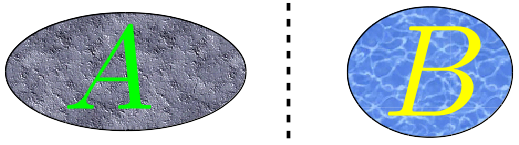
\includegraphics[width=0.5\linewidth]{./pic/algo_sets_simple} };}
    
   % {\small Для нахождения $\P(A)$ перебор всех векторов $t$ потребовал бы $O(\abs{X}^{nm})$ операций!}
    Разработан алгоритм, который за время $O(nm)$ позволяет проверить, пересекаются ли $\Eps(d)$ и $B$. Если и только если пересекаются, $\P(\Eps(d)) > p_0$.
\end{center}
\begin{tikzpicture}[overlay]
	\path[->] (nPA.south) edge [bend right] (tSets.west);
	\path[->] (nB.south) edge (tSets.north north east);
\end{tikzpicture}
\end{frame} %===========================

% == eof == eof ===
\section{Задача и алгоритм коллективной экспертизы}

\begin{frame}{Задача коллективной экспертизы: варианты}
 \vspace*{-3mm}
	\begin{enumerate}
		\item Методы Ю.~П.~Пытьева\footnote{Пытьев\;Ю.\,П. \emph{Эмпирическое восстановление мер возможности и правдоподобия возможности в моделях экспертных решений}, 2009}:
% .}~// Докл. АН СССР, Т.\;224, \No 6, С.\;1283--1286, 2009.\\}: 
		матрицы попарных сравнений и др.;
		\item Новый метод -- вектора предпочтений; %новый для т.\,в.~Пытьева
		\item Новый метод -- введение отношения предпорядка (частичного порядка с точностью до эквивалентности) на множестве распределений нечёткого элемента, вычислние (точной) верхней/нижней грани распределений.
	\end{enumerate} 
	
	{ \small Коллективное мнение экспертов с помощью матриц попарного сравнения: 
	\\ $\big(  \p^{(r)}(\cdot)$ -- совместное распределение на основе оценок эксперта $r = 1 \ldots R \big)$ 
	\begin{columns}
	   \column{0.5\textwidth}
	      \begin{gather*}
		   m^{(r)}_{kj} = \begin{cases}
			\;\;\;1,\;\; \p^{(r)}(t_k) > \p^{(r)}(t_j)\\
			\;\;\;0,\;\; \p^{(r)}(t_k) = \p^{(r)}(t_j)\\
			-1, \;\; \p^{(r)}(t_k) < \p^{(r)}(t_j)
		  \end{cases} 
		  \\ k,j = 1\ldots\abs{T}+1; 
		  \\ \text{причём }\p^{(r)}(t_{\abs{T}+1}) \define= 0.  
	      \end{gather*}
	   \column{0.5\textwidth}
	     \vspace*{-3mm}
	      \begin{gather*}
		  m_* = \arg \min_m \sum_{r=1}^{R} \rho(m^{(r)}, m),
		  \\ \text{где } \rho(m, m') = \big( \sum_{k,j=1}^{\abs{T}+1}(m_{kj} - {m'}_{kj})^2 \big)^{1/2}.
		  \\ \text{$m_*$ не всегда просто найти!}
	      \end{gather*}
	\end{columns}  } 
\end{frame} %===========================

\begin{frame}{Вектора предпочтений}
	\vspace{-3mm}
	{ \small Коллективное мнение экспертов с помощью векторов предпочтений аналогично случаю матриц парных сравнений ($r = 1 \ldots R$):}
	\begin{gather*}
		s^{(r)}_j = \sum_{t \in T} \mathlarger{\mathlarger{\chi} }_{A_j^{(r)}}(t),
		 \mathsmaller{\text{\small причём } \p^{(r)}(t_{\abs{T}+1}) \define= 0, \; j = 1\ldots\abs{T}+1. } 
		 \\ \text{Здесь } A^{(r)}_j = \{t \in T: \p^{(r)}(t) \leq \p^{(r)}(t_j)\}. 
	\end{gather*}
	Вектор предпочтений $s$ должен удовлетворять двум условиям:
	\\ (1) $\max s_j= |T|$ (нормировка возможности);
	\\ (2) число координат $|J_i| = i$, где $J_i = \{j: s_j \leq i\}$, $i \subset I = \{1 \ldots |T|\}$.
	
	\textbf{Задача}: $\displaystyle s_* = \arg \underset{s} \min \sum_{r=1}^R \rho(s - s^{(r)})$, где  $\displaystyle \rho(s, s') = \big( \sum_{j=1}^{\abs{T}+1}(s_{j} - {s'}_{j})^2 \big)^{1/2}$.
	
	\textbf{Алгоритм решения}:  берём  $ \ol s =  \frac{1}{R} \sum_{r=1}^R s^{(r)}$ и удовлетворяем условия (1-2), изменяя как можно меньше  координат на как можно меньшую величину.
\end{frame} %===========================

   % \begin{tikzpicture}
  %    \begin{axis}[
%	width = 0.5\textwidth, height = 0.4\textwidth,
 %   xlabel = {$L$},
%    ylabel = {$\alpha$},
	%ymin = 0, ymax = 0.4,  % if left default there will be margins
	%xmin = 2, xmax = 30,
 %   xtick = {2, 6, 10, 14, 18, 22, 26, 30}
%	xticklabels = {,,},
%	yticklabels = {,,}
%	]
%	\addplot[blue, very thick] table[x=n, y=cone] {./pic/results.txt};
%	\addplot[dash pattern=on 6pt off 3pt on 1pt off 3pt] table[x=n, y=svm] {./pic/results.txt};
%     \end{axis}
 %   \end{tikzpicture}


\begin{frame}{Предпорядок распределений возможности}
	\begin{columns}
	  \column{0.6\textwidth}
	    \begin{gather*}
	    \p_1 \prec \p_2 \text{ (читается <<уточняет>>) } \Leftrightarrow \\ 
	     \Leftrightarrow
	    \begin{cases}
 		  \supp\;p_2 \supset \supp \; \p_1;
		  \\ \exists \gamma: \p_2(\omega) = \gamma(\p_1(\omega))\;   \mathsmaller{ \omega \in \supp\;\p_1}; 
		 \\ \mathsmaller{\gamma: \zo \rightarrow \zo \text{ -- монотонная непрерывная,} } 
		%  \\ \hspace{10ex}
		\mathsmaller{\gamma(0)=0, \gamma(1)=1}
		 \\ p_2(\omega) \leq p_2(\omega'),  \mathsmaller{\omega \not\in  \supp \; \p_1,  \omega' \in  \supp \; \p_1}.
	    \end{cases}
	    \end{gather*}
	    

	    \begin{center}
		При достаточно общих условиях: %множества решений {\em задачи выбора} вложены:
		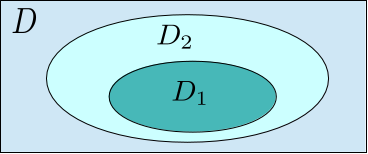
\includegraphics[width=0.75\linewidth]{./pic/solution_sets2}
		%\\ Здесь $D = 2^{\setN}$,
		\\ $\displaystyle D_r = \arg \min_d \P^{(r)}(\Eps(d))$ {\footnotesize -- решения задачи выбора на оценках $r$-го эксперта, $D$ -- все решения.}  
	     \end{center}
	  
	  \vspace*{-1mm}	   
	   {\small Оправдано использование $\p_1 \vee \p_2$ (супремума).} 
%	    \begin{gather*}
%		\mathsmaller{  \check{\p} \succ \p_1, \check{\p} \succ \p_2 }, \text{но: } \\ \forall\;\p' \neq \check{\p}, \p' \succ \p_1, \p' \succ \p_2: \p' \succ \check{\p}.
%	    \end{gather*}
	    
	%    \vspace*{2mm}
	  %  \emph{Опр.} $\hat{\p} = \p_1 \wedge \p_2$ (<<инфинум>>) -- аналогично.
	     
	%     \vspace*{1mm}

	   \column{0.4\textwidth}
	     \begin{center}
	     	\hspace*{-2mm}    \tikz{ \node (otriv){   
      \begin{tikzpicture}  \begin{axis}[width = 35mm, height = 25mm,	xticklabels = {,,}, yticklabels = {,,}, ymin = -0.1, ymax = 1.1 ]
	\addplot[green, ultra thick] table[x=xx, y=triv] {./pic/chapeter02-lattice2.dat};
       \end{axis}   \end{tikzpicture} };}
	     	    \vspace{2mm} 
		\\ \hspace*{-3mm} \tikz{ \node (osup){   
      \begin{tikzpicture}  \begin{axis}[width = 35mm, height = 25mm,	xticklabels = {,,}, yticklabels = {,,}, ymin = -0.1, ymax = 1.1 ]
	\addplot[green, very thick] table[x=xx, y=sup] {./pic/chapeter02-lattice2.dat};
       \end{axis}   \end{tikzpicture}  };}
	    \end{center} 
	     \vspace{-3mm}
	     \begin{columns}
		  \column{0.5\linewidth}
		   \begin{center}
		      \tikz{ \node (oPP1){   
      \begin{tikzpicture}  \begin{axis}[width = 35mm, height = 25mm,	xticklabels = {,,}, yticklabels = {,,}, ymin = -0.1, ymax = 1.1 ]
	\addplot[green, very thick] table[x=xx, y=pp1] {./pic/chapeter02-lattice2.dat};
       \end{axis}   \end{tikzpicture} };}
		     \vspace{-2mm}
		  \\ \tikz{ \node (oP1){   
      \begin{tikzpicture}  \begin{axis}[width = 35mm, height = 25mm,	xticklabels = {,,}, yticklabels = {,,}, ymin = -0.1, ymax = 1.1 ]
	\addplot[green, very thick] table[x=xx, y=p1] {./pic/chapeter02-lattice2.dat};
       \end{axis}   \end{tikzpicture} };}
		   \end{center} 
		  \column{0.5\linewidth}
		   \begin{center}
		     \tikz{ \node (oPP2){   
      \begin{tikzpicture}  \begin{axis}[width = 35mm, height = 25mm,	xticklabels = {,,}, yticklabels = {,,}, ymin = -0.1, ymax = 1.1 ]
	\addplot[green, very thick] table[x=xx, y=pp2] {./pic/chapeter02-lattice2.dat};
       \end{axis}   \end{tikzpicture} };}
		      \vspace{-2mm}
		  \\ \tikz{ \node (oP2){   
      \begin{tikzpicture}  \begin{axis}[width = 35mm, height = 25mm,	xticklabels = {,,}, yticklabels = {,,}, ymin = -0.1, ymax = 1.1 ]
	\addplot[green, very thick] table[x=xx, y=p2] {./pic/chapeter02-lattice2.dat};
       \end{axis}   \end{tikzpicture} };}
		   \end{center} 
	      \end{columns}
	      \begin{center}
	          \vspace{-2ex}
		 {\small  Распределения образуют полурешётку. }
	     \end{center}
	\end{columns}
	
	\begin{tikzpicture}[overlay]
		\path[->] (otriv.south) edge  (osup.north);
		\path[->] (osup.south) edge  (oPP1.north);
		\path[->] (osup.south) edge  (oPP2.north);
		\path[->] (oPP1.south) edge  (oP1.north);
		\path[->] (oPP2.south) edge  (oP2.north);
	\end{tikzpicture}	
\end{frame} %===========================



\begin{frame}{Алгоритм коллективной экспертизы}
 \begin{center}
    Пусть имеется $n$ объектов с $m$ параметрами, и $R$ экспертов, каждый из которых оценил все объекты по всем параметрам (если это не так, отсутствующие распределения считаем тривиальными.)
	\\ \vspace{3mm} \textbf{Идея}: 
	\begin{enumerate}
		\item составить <<длинные>> вектор $(\p_{11}^{(1)}, \ldots \p_{nm}^{(1)});\; (\p_{11}^{(2)}, \ldots \p_{nm}^{(2)})$ и т.\,д.;
		\item рассчитать коллективный вектор $(\p_{11}, \ldots \p_{nm})$ методом $\vee$ или методом матриц п.\,с.;
		\item Одномерные <<куски>> этого вектора, $\p_{ij}$,  считать коллективным мнением экспертов по параметрам объектов {\footnotesize $i = 1 \ldots n$, $j = 1 \ldots m$}. 
	\end{enumerate}	
 \end{center}
\end{frame} %===========================

% == eof == eof ===
 
\section{Результаты}
\begin{frame}{Пример решения задачи  коллективной экспертизы}
  \vspace{-2ex}
  \begin{center}
    Графики $\p_1, \p_2$ -- исходные распределения, $\p$ -- их супремум, $\check{\p}$ -- их верхняя грань, вычисленная по <<быстрому>> алгоримту.
      \vspace{-1ex}
    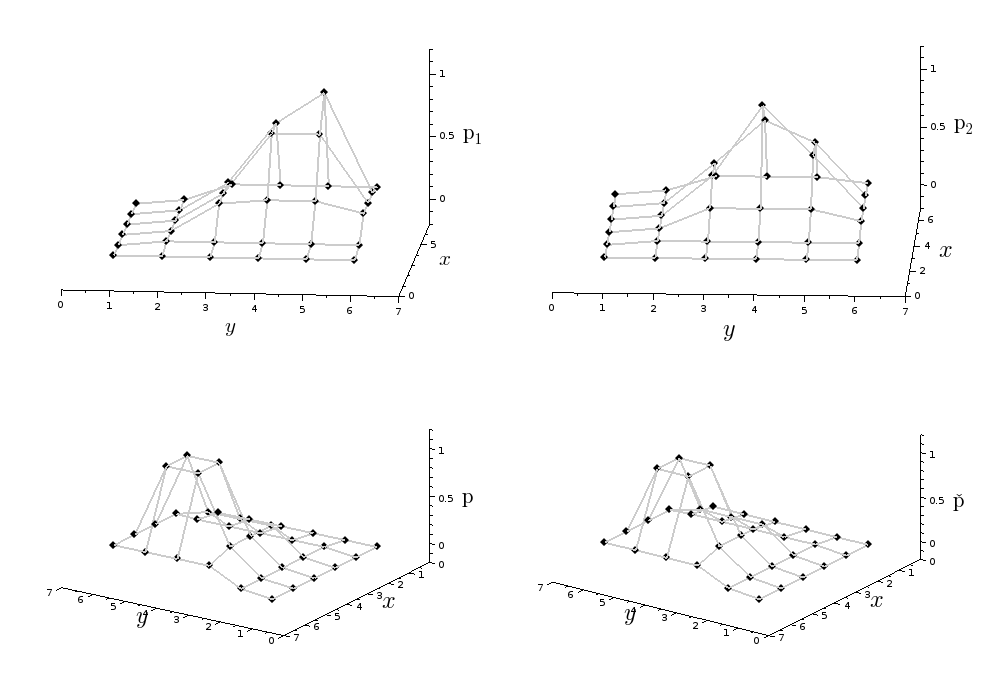
\includegraphics[width=0.8\linewidth]{./pic/myplot_sovp}
  \end{center} 
\end{frame} %===========================

\begin{frame}{Пример решения задачи  коллективной экспертизы}
  \vspace{-2ex}
  \begin{center}
    Графики $\p_1, \p_2$ -- исходные распределения, $\p$ -- их супремум, $\check{\p}$ -- их верхняя грань, вычисленная по <<быстрому>> алгоримту.
      \vspace{-1ex}
    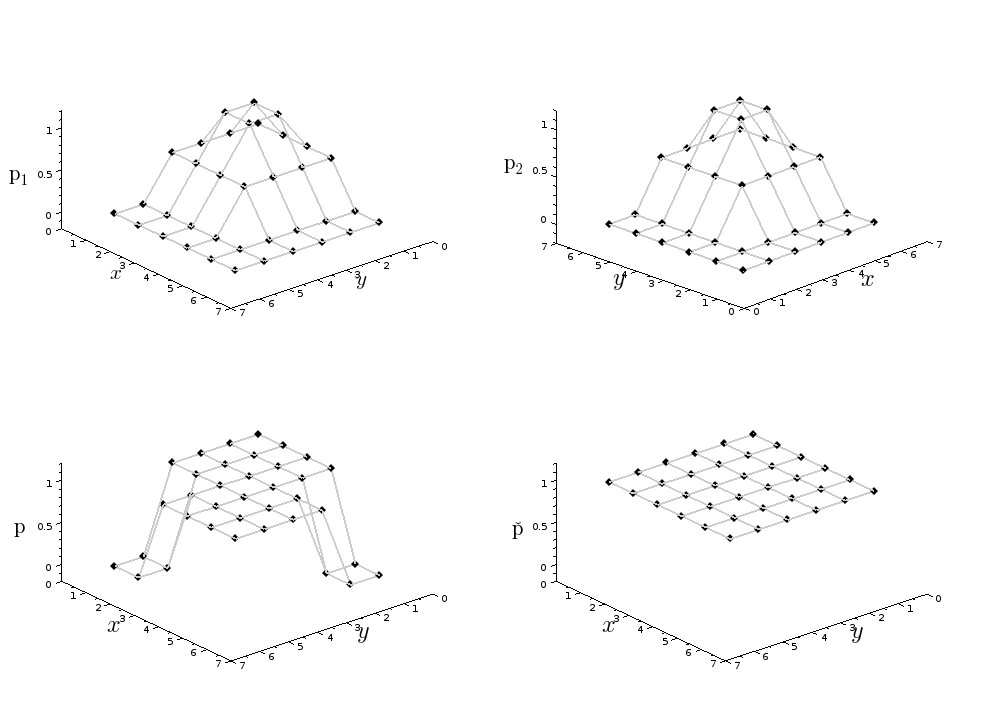
\includegraphics[width=0.8\linewidth]{./pic/mytest}
  \end{center} 
\end{frame} %===========================

\begin{frame}{Примеры решений задачи  коллективной экспертизы}
  \vspace{-2ex}
  \begin{center}
    Графики $p_1, p_2, p_3$ -- исходные распределения, $\bar{\p}$ -- среднее, вычисленное по методу векторов предпочтений, $\p$ -- супремум. 
  \end{center} 
  \vspace{-3ex}
  \begin{columns}
    \column{0.55\textwidth}
	  \begin{center}
	      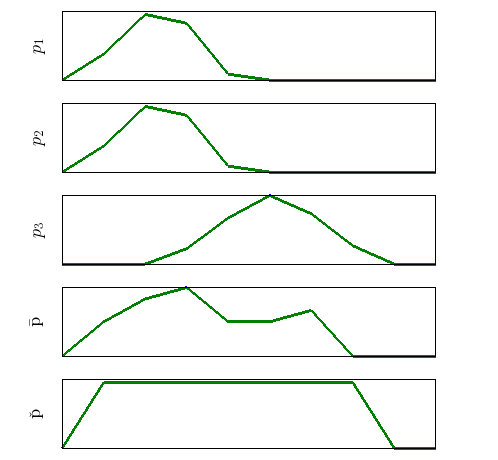
\includegraphics[width=0.9\linewidth]{./pic/prefsup102}
	  \end{center}
    \column{0.50\textwidth}
          \begin{center}
	      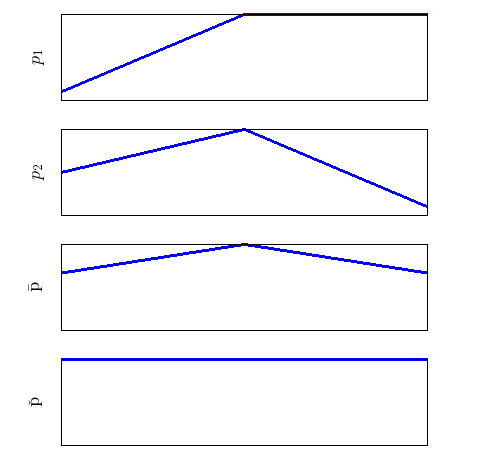
\includegraphics[width=1\linewidth]{./pic/prefsup6}
	  \end{center}
  \end{columns}
\end{frame} %===========================

\begin{frame}{Пример модели <<качества>> объекта}
	\begin{center}
		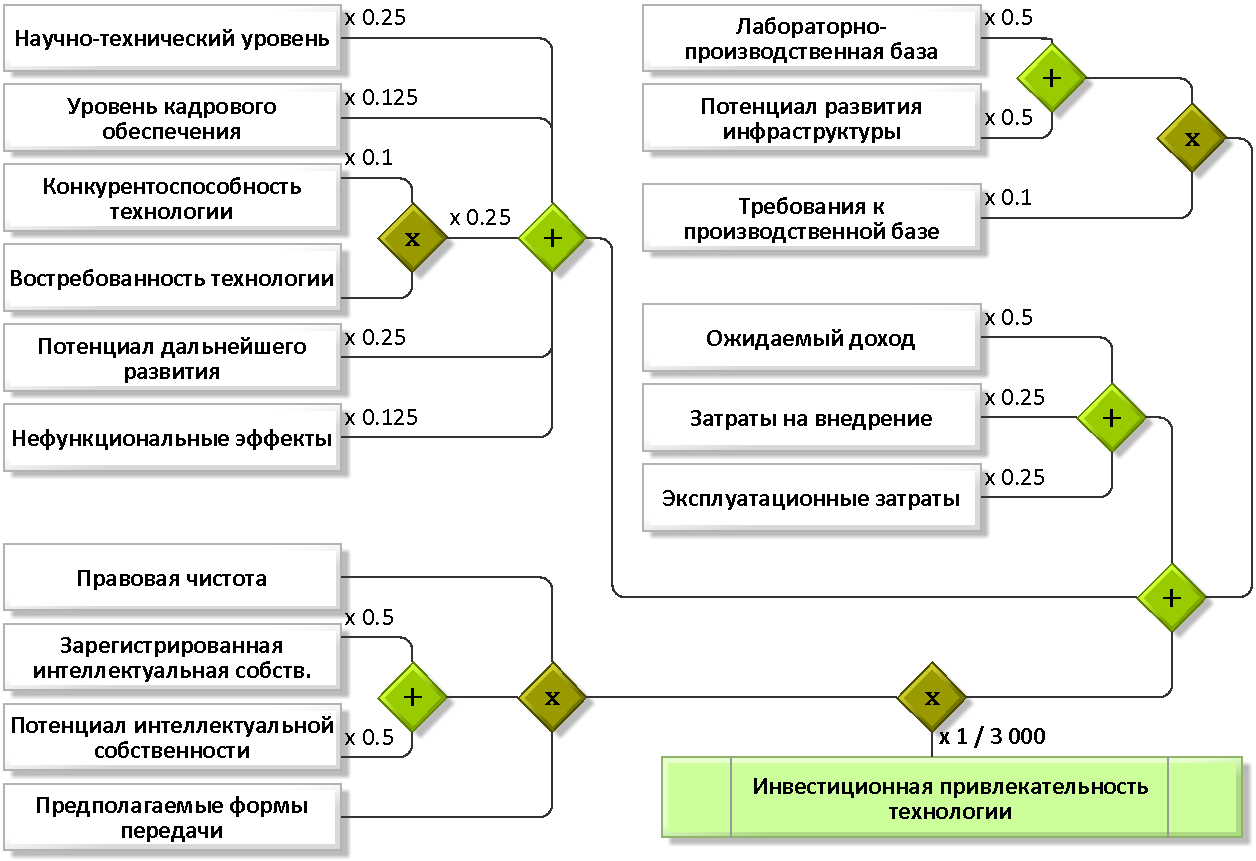
\includegraphics[width=0.85\linewidth]{./pic/schemeF2}
	\end{center}
\end{frame} %===========================

\begin{frame}{Примеры решений задачи выбора}
 \begin{center}
	\begin{columns}
	 \column{0.50\textwidth}  
	 \vspace{-1ex}
	 \begin{equation*}
	    n = 15, m = 16,  f: \text{см. блок-схему}.
	 \end{equation*}
	  \vspace{-4ex}
	  {
	      \\[0.5ex] \hspace{2ex} Для k=2  :  6 7; 
	      \\[0.5ex] \hspace{2ex} Для k=14:  все, кроме 13; 
	      \\[0.5ex] \hspace{2ex} Для остальных k -- неоднозначно.
	  }
	  \vspace{1ex}
	  \begin{center}
	    \resizebox{0.7\linewidth}{!}{\showevDisplayFullScale{./pic/realScaled13.txt}}
	  \end{center} 
	 \column{0.45\textwidth}
	  \begin{equation*}
	    \hspace{-2ex} n = 3, m = 1, f(x) = x.
	  \end{equation*}
	  \\ \vspace{1ex}
	      \resizebox{0.9\linewidth}{!}{\showevDisplay{./pic/sample1/ex1.txt}}
	      \\ \hspace{2ex} Ранжировка (Э1): $1, 2, 3$.
		  \\ \vspace{1ex}
	      \resizebox{0.9\linewidth}{!}{\showevDisplayRough{./pic/sample1/ex2.txt}}
	      \\ \hspace{2ex} Ранжировка (Э2): $3, 2, 1$.	      
		  \\ \vspace{1ex}
	      \resizebox{0.9\linewidth}{!}{\showevDisplayRough{./pic/sample1/mean.txt}}
	      \\ \hspace{2ex}  Ранжировка (среднее): $2, 3, 1$.
		  \\ \vspace{1ex}
	      \resizebox{0.9\linewidth}{!}{\showevDisplayRough{./pic/sample1/sup.txt}}
	      \\ \hspace{2ex} Ранжировка (супремум): \textbf{?}	     
	
	\end{columns}
 \end{center}
\end{frame} %===========================

\begin{frame}{Пользовательский интерфейс}
          \begin{center}
	      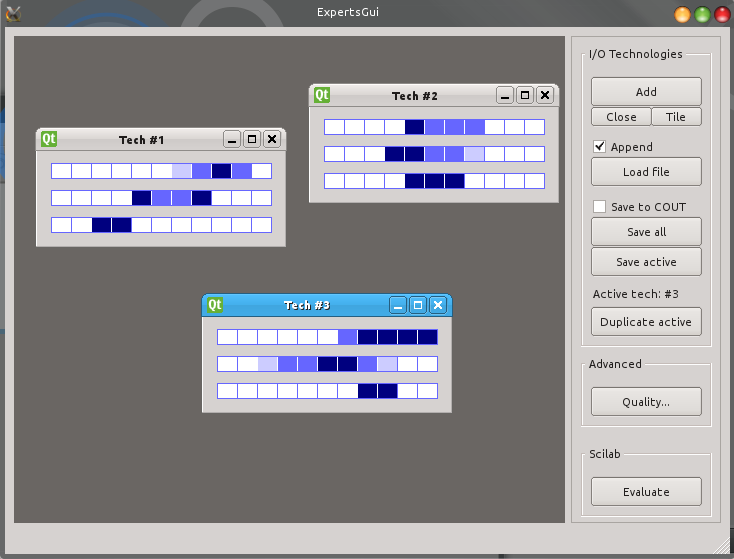
\includegraphics[width=0.75\linewidth]{./pic/combination6}
	  \end{center}
\end{frame} %===========================
% == eof == eof ===


% === final slide ====
\begin{frame}{Спасибо за внимание!}
	\begin{center}
		
\includegraphics[width=0.5\linewidth]{./pic/biber_final}
	\end{center}
\end{frame}
% =============

\end{document}
